%% ============================================================
%%  SIC-AI Capstone — Mid-Term Progress Report
%%  Speaker-Aware Noise Cancellation and Target Speech Enhancement
%%
%%  Build:  latexmk -pdf main.tex
%%  Search for "TODO" to find every item that still needs a source.
%%  Set \showtodofalse only when every TODO has been resolved.
%% ============================================================
\documentclass[11pt,a4paper]{article}

\usepackage[T1]{fontenc}
\usepackage[utf8]{inputenc}
\usepackage{lmodern}
\usepackage[margin=2.4cm]{geometry}
\usepackage{microtype}
\usepackage{amsmath,amssymb}
\usepackage{graphicx}
\usepackage{booktabs,tabularx,array,multirow}
\usepackage{xcolor}
\newcolumntype{Y}{>{\raggedright\arraybackslash}X}
\usepackage{caption,subcaption}
\usepackage{enumitem}
\usepackage{float}
\usepackage{tikz}
\usetikzlibrary{positioning,arrows.meta,fit,calc}
\usepackage[numbers,sort&compress]{natbib}
\usepackage{fancyhdr}
\usepackage{setspace}
\usepackage[hidelinks]{hyperref}
\usepackage[nameinlink]{cleveref}

\setstretch{1.06}
\setlength{\parskip}{3.5pt}
\setlength{\parindent}{0pt}
\captionsetup{font=small,labelfont=bf,skip=4pt}
\setlist{itemsep=1.5pt,topsep=3pt}
\graphicspath{{figures/}}

% ---------- TODO markers ----------
\newif\ifshowtodo
\showtodofalse      % all source-backed TODOs have been resolved
\newcommand{\todo}[1]{\ifshowtodo{\color{red}\textbf{[TODO: #1]}}\fi}

% ---------- shortcuts ----------
\newcommand{\sisdr}{SI-SDR}
\newcommand{\sisdri}{SI-SDRi}
\newcommand{\spk}{\mathbf{e}}
\newcommand{\done}{\textbf{Done}}
\newcommand{\partl}{\textbf{Partial}}
\newcommand{\pending}{\textbf{Pending}}
\newcommand{\inprog}{\textbf{In progress}}

% ---------- header / footer ----------
\pagestyle{fancy}
\fancyhf{}
\lhead{\small SIC-AI Capstone: Mid-Term Progress Report}
\rhead{\small Speaker-Aware Noise Cancellation}
\cfoot{\small\thepage}
\renewcommand{\headrulewidth}{0.3pt}

\begin{document}

%% ============================================================
%%  TITLE PAGE
%% ============================================================
\begin{titlepage}
\thispagestyle{empty}
\centering
{\Large\bfseries Samsung Innovation Campus\par}
\vspace{2mm}
{\large Enabling People Together\par}
\vspace{10mm}

\includegraphics[height=3.0cm]{tu_logo.png}\par
\vspace{8mm}
{\large Tribhuvan University\par}
\vspace{2mm}
{\large Pulchowk Campus\par}
\vspace{10mm}
{\large SIC-AI Capstone Project\par}
\vspace{2mm}
{\LARGE\bfseries Mid-Term Progress Report\par}
\vspace{12mm}
{\LARGE\bfseries Speaker-Aware Noise Cancellation\\ and Target Speech Enhancement\par}
\vspace{14mm}
{\large\bfseries Submitted By\par}
\vspace{3mm}
\begin{tabular}{@{}ll@{}}
Austina Aryal & (079BEI010)\\
Prashamsa Aryal & (079BEI024)\\
Sostika Shrestha & (079BEI041)
\end{tabular}
\vspace{10mm}

{\large\bfseries Submitted To\par}
\vspace{2mm}
{\large Arun Timilsena and Suresh Pokharel\par}
{\small Supervisors, SIC-AI Capstone Project\par}
\vfill
{\large November 2026 (Kartik 2083)\par}
\end{titlepage}
\setcounter{page}{2}

%% ============================================================
%%  ABSTRACT
%% ============================================================
\section*{Abstract}
We are building a target speaker extraction system for our SIC-AI capstone. The input is a
single-channel recording that may contain the target speaker, another talker and background noise,
together with a short enrollment recording of the target; the output should contain only the
target's voice. The proposal combined a frozen ECAPA-TDNN speaker encoder with a causal
Conv-TasNet/BSRNN separator. During implementation we dropped Conv-TasNet and kept a
speaker-conditioned BSRNN with 16.83\,M parameters. A frozen ECAPA-TDNN produces a
192-dimensional embedding, which is added once to the band features and injected through FiLM in
each of the eight dual-path layers. The model is trained on on-the-fly mixtures of LibriSpeech
speech and DEMAND noise with a combined \sisdr{} and multi-resolution STFT loss.

Training finished all 100 epochs. Validation \sisdri{} on unseen speakers rose from 8.1\,dB at
epoch~33 to a best of 11.84\,dB at epoch~97. On the 1200-mixture test set, the earlier-checkpoint
evaluation gives a 10.8\,dB \sisdr{} gain and raises STOI from 0.77 to 0.87 on non-clean mixtures;
a Whisper check on the final checkpoint lowers word error rate from 38.3\% to 18.1\%. The model
chooses the wrong speaker in 7.7\% of interferer mixtures, mostly when enrollment is short. It is
non-causal, and the test tables still need to be rerun with the final checkpoint. Remaining work
covers that rerun, the conditioning ablation, an unseen-noise test and CPU measurements.

\newpage
\begingroup
\small
\setlength{\parskip}{0pt}
\tableofcontents
\endgroup
\newpage

%% ============================================================
%%  1. INTRODUCTION
%% ============================================================
\section{Introduction}

\subsection{Problem and motivation}
Conventional noise suppression removes environmental noise but treats every human voice as
signal. In a call or a meeting, a second person talking nearby is not noise in that sense, yet is
still unwanted. Target speaker extraction (TSE) handles this by conditioning the enhancement
network on an enrollment recording of the desired speaker, so that only that voice is kept
\cite{wang2019voicefilter, sato2024speakerbeamss}. Because the output is tied to one enrolled
speaker, TSE avoids the permutation problem of blind speech separation and does not need to know
how many speakers are present.

\subsection{Objectives}
The proposal set three objectives:
\begin{enumerate}
  \item design and implement a target-speaker extraction system that combines a pretrained speaker
        encoder with a separator network;
  \item evaluate quality, generalisation and efficiency (\sisdr, STOI, PESQ, unseen speakers and
        noise, model size and compute);
  \item deliver a reproducible training and evaluation framework.
\end{enumerate}

\subsection{Scope of this report}
This report records what has been completed against the proposal timeline, how and why the design
changed, the current system and data, the results so far, and the remaining work and risks.

%% ============================================================
%%  2. PROGRESS AND CHANGES
%% ============================================================
\section{Progress and Changes from the Proposal}
\label{sec:changes}

\Cref{tab:progress} compares the work packages in the proposal timeline with their current status.

\begin{table}[htbp]
\centering\footnotesize
\caption{Status of the proposal work packages at mid-term.}
\label{tab:progress}
\begin{tabularx}{\textwidth}{@{}>{\raggedright\arraybackslash}p{4.3cm} l Y@{}}
\toprule
\textbf{Work package} & \textbf{Status} & \textbf{Notes}\\
\midrule
Literature review and dataset survey & \done &
  Reviewed in the proposal and extended with BSRNN and dual-path work (\Cref{sec:related}).\\
Audio pipeline and classical baseline & \partl &
  STFT/iSTFT pipeline done. The classical baseline was not evaluated; the supplied code and logs
  contain no baseline implementation or result.\\
Dataset preparation and mixture generation & \done &
  LibriSpeech and DEMAND manifests, fixed validation and test sets, on-the-fly scene sampler
  (\Cref{sec:data}).\\
ECAPA-TDNN encoder and conditioning ablation & \partl &
  Frozen ECAPA-TDNN with cached embeddings done; additive and FiLM conditioning implemented.
  The concat/FiLM/gating ablation is not done.\\
Separator backbones & \partl &
  Conv-TasNet reached 5.90\,dB validation \sisdri{} at epoch 21 before being dropped;
  speaker-conditioned BSRNN trained for 100 epochs (\Cref{sec:changes}). TF-GridNet not
  attempted.\\
Curriculum training and augmentation & \partl &
  Randomised scenarios, SIR/SNR and levels. No curriculum schedule and no reverberation yet.\\
Evaluation and generalisation tests & \inprog &
  Test metrics, scenario/SNR/SIR breakdowns, speaker confusion and WER are documented
  (\Cref{sec:results}); the final-checkpoint rerun, ablations and unseen-noise tests are pending.\\
Latency, CPU and memory optimisation & \partl &
  GPU cost measured offline (RTF 0.028, 16.83\,M parameters). CPU speed and causal latency are
  not measured; the model is non-causal.\\
Final validation and documentation & \pending &
  This report is the first documentation milestone.\\
\bottomrule
\end{tabularx}
\end{table}

The main achievements so far are: a speaker-conditioned BSRNN with 16.83\,M parameters, trained
for the full 100 epochs, with a best validation \sisdri{} of 11.84\,dB at epoch~97 on unseen
speakers; an earlier-checkpoint test evaluation with a 10.8\,dB \sisdr{} gain, STOI rising from
0.77 to 0.87 and PESQ 2.20 on non-clean mixtures; a Whisper word error rate falling from 38.3\% to
18.1\%; a measured speaker-confusion rate of 7.7\%; and a resumable training pipeline with cached
embeddings, fixed manifests and an inference path that accepts a user's own mixture and enrollment
recording.

\subsection{Design changes}
The largest change was the separator backbone. The proposal put Conv-TasNet first and BSRNN
second. We trained a causal Conv-TasNet with $N=512$, $H=512$, film2 conditioning, 3\,s segments,
batch 3 with gradient accumulation 2, and learning rate $10^{-3}$ for a planned 80 epochs. The
saved best checkpoint is epoch~21 with validation \sisdri{} 5.90\,dB; a 20-clip check gave
3.88\,dB on training voices and 3.60\,dB on held-out voices and noise. We dropped it because
BSRNN reached 11.84\,dB validation \sisdri{}. \Cref{tab:changes} lists the other deviations.

\begin{table}[htbp]
\centering\footnotesize
\caption{Differences between the proposal and the current implementation.}
\label{tab:changes}
\begin{tabularx}{\textwidth}{@{}l Y Y Y@{}}
\toprule
\textbf{Aspect} & \textbf{Proposal} & \textbf{Current} & \textbf{Reason}\\
\midrule
Separator & Causal Conv-TasNet; BSRNN as a stretch goal & Speaker-conditioned BSRNN, 8 dual-path layers & Conv-TasNet reached 5.90\,dB validation \sisdri, below BSRNN's 11.84\,dB\\
Causality & Strictly causal (past and current frames) & Non-causal (bidirectional LSTMs) & Causal operation is deferred\\
STFT & 512-point FFT, 160-sample hop (10\,ms) & 512-point FFT, 128-sample hop (8\,ms) & Finer time resolution for BSRNN\\
Speaker encoder & ECAPA-TDNN, frozen versus fine-tuned & Frozen ECAPA-TDNN, cached embeddings & Saves GPU time and memory\\
Data & VoiceBank, DEMAND, MUSAN, DNS & LibriSpeech (1172 training speakers) and 16 DEMAND environments & Many clean speakers; one noise source\\
Reverberation & Limited RIR simulation & Not included yet & Listed as future work\\
Loss & \sisdr{} + spectral + mask terms & \sisdr{} (clamped at 30\,dB) + 5$\times$ multi-resolution STFT & Waveform and spectral objective; mask term dropped\\
Test protocol & Speaker- and noise-disjoint sets & Speaker-disjoint; noise audio disjoint, environments shared & See \Cref{sec:limits}\\
\bottomrule
\end{tabularx}
\end{table}

%% ============================================================
%%  3. BACKGROUND
%% ============================================================
\section{Background and Related Work}
\label{sec:related}

\paragraph{Target speaker extraction.}
VoiceFilter \cite{wang2019voicefilter} conditions a spectrogram mask estimator on a d-vector of the
target speaker. SpeakerBeam-SS \cite{sato2024speakerbeamss} uses lightweight Conv-TasNet variants
with state-space modelling for low-latency operation. We use the same enrollment-conditioned
formulation but a band-split time--frequency backbone.

\paragraph{Band-split RNN.}
BSRNN \cite{luo2023bsrnn} splits the complex spectrogram into sub-bands, projects each band to a
common feature size and alternates RNNs along time and along bands, in the spirit of dual-path
models \cite{luo2020dprnn}. It was first used for music separation and later for efficient speech
enhancement \cite{yu2023efficient}. TF-GridNet \cite{wang2023tfgridnet} is a heavier alternative
that we keep as a possible upper-bound reference.

\paragraph{Speaker embeddings and conditioning.}
ECAPA-TDNN \cite{desplanques2020ecapa} maps an utterance to a fixed-length speaker embedding; we
use the SpeechBrain implementation \cite{ravanelli2021speechbrain}. Feature-wise linear modulation
(FiLM) \cite{perez2018film} scales and shifts feature channels from a conditioning vector and is
our main speaker-injection mechanism.

\paragraph{Losses and metrics.}
We optimise scale-invariant SDR \cite{leroux2019sdr} with a multi-resolution STFT loss
\cite{yamamoto2020pwg}, and evaluate with \sisdri, STOI \cite{taal2011stoi} and wideband PESQ
\cite{itu2007p8622}. The DNS Challenge \cite{reddy2020dns} and DeepFilterNet
\cite{schroter2022deepfilternet} motivated the original efficiency goals.

%% ============================================================
%%  4. SYSTEM DESIGN
%% ============================================================
\section{Current System Design}
\label{sec:system}

\subsection{Overview}
Given a mixture $x = s_t + s_i + n$ (target, interferer, noise) and an enrollment embedding
$\spk\in\mathbb{R}^{192}$ of the target, the network predicts a complex mask $M$ on the mixture
spectrogram $X$ and returns $\hat{s}_t = \mathrm{iSTFT}(M\odot X)$. \Cref{fig:arch} shows the
pipeline.

\begin{figure}[t]
\centering
\resizebox{\textwidth}{!}{%
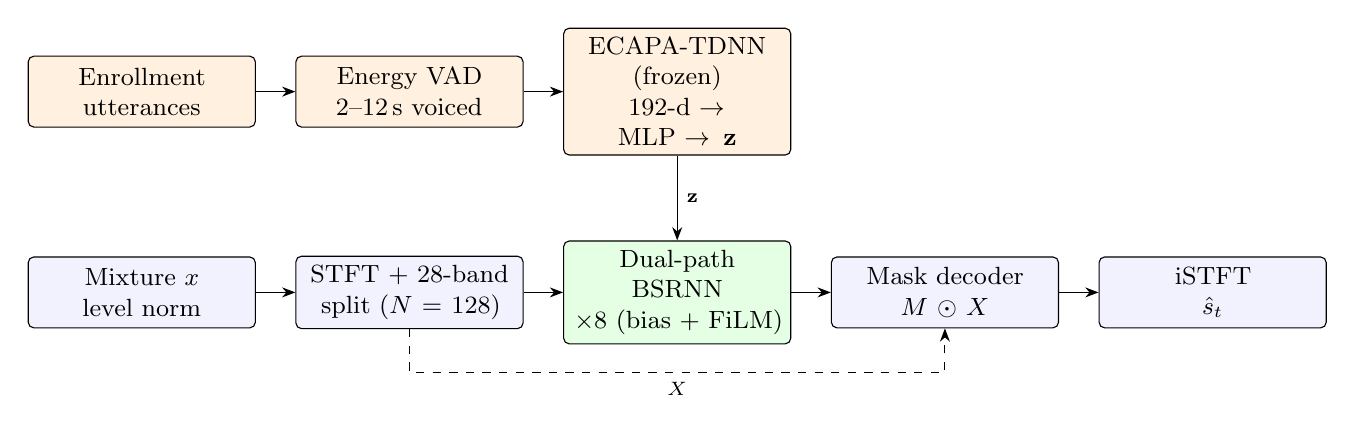
\begin{tikzpicture}[
  x=1cm,y=1cm,
  box/.style={draw,rounded corners=2pt,align=center,font=\small,minimum height=9mm,
              text width=2.65cm,fill=blue!5},
  spk/.style={draw,rounded corners=2pt,align=center,font=\small,minimum height=9mm,
              text width=2.65cm,fill=orange!12},
  >=Stealth]
% speaker branch
\node[spk] (enr)   at (0.0,2.55) {Enrollment\\utterances};
\node[spk] (vad)   at (3.4,2.55) {Energy VAD\\2--12\,s voiced};
\node[spk] (ecapa) at (6.8,2.55) {ECAPA-TDNN (frozen)\\192-d $\to$ MLP $\to \mathbf{z}$};
% signal path
\node[box] (mix)   at (0.0,0) {Mixture $x$\\level norm};
\node[box] (fe)    at (3.4,0) {STFT + 28-band\\split ($N=128$)};
\node[box,fill=green!10] (bsrnn) at (6.8,0) {Dual-path BSRNN\\$\times 8$ (bias + FiLM)};
\node[box] (dec)   at (10.2,0) {Mask decoder\\$M\odot X$};
\node[box] (out)   at (13.6,0) {iSTFT\\$\hat{s}_t$};
\draw[->] (enr) -- (vad);
\draw[->] (vad) -- (ecapa);
\draw[->] (ecapa.south) -- (bsrnn.north) node[midway,right,font=\scriptsize]{$\mathbf{z}$};
\draw[->] (mix) -- (fe);
\draw[->] (fe) -- (bsrnn);
\draw[->] (bsrnn) -- (dec);
\draw[->] (dec) -- (out);
\draw[->,dashed] (fe.south) -- ++(0,-0.55) -| (dec.south)
  node[pos=0.25,below,font=\scriptsize]{$X$};
\end{tikzpicture}%
}
\caption{Speaker-conditioned BSRNN. The speaker vector $\mathbf{z}$ is added once to the band
features and used by FiLM in every dual-path layer. The dashed path carries the mixture
spectrogram to the mask multiplier.}
\label{fig:arch}
\end{figure}

\subsection{Front end and band split}
Audio is processed at 16\,kHz. The waveform is divided by its standard deviation, and the output
is multiplied back, so the network sees level-independent input. An STFT with a 512-point Hann
window (32\,ms) and a 128-sample hop (8\,ms) gives 257 complex bins per frame; a 4\,s training clip
yields 501 frames. STFT, iSTFT and the loss are computed in fp32 even under mixed precision.

The 257 bins are grouped into 28 non-uniform bands: 8 bands of 125\,Hz below 1\,kHz, 12 bands of
250\,Hz between 1 and 4\,kHz, and 8 bands of 500\,Hz between 4 and 8\,kHz. The last band takes the
one leftover bin. For each band, the real and imaginary parts are layer-normalised and linearly
projected to $N=128$ features, producing a tensor of shape $[B,28,T,N]$. The fine low-frequency
resolution follows the harmonic structure of speech; the coarser high-frequency bands cost less
and carry less formant information.

\subsection{Speaker branch and conditioning}
Enrollment audio is cleaned with an energy-based voice activity detector (25\,ms frames, 10\,ms
hop, threshold 30\,dB below the 95th-percentile frame energy, floor $-55$\,dB, 10-frame hang). The
same VAD is used when building the cached enrollment banks and in \texttt{embed\_enrollment} for a
user's own recording. Voiced speech from several of the speaker's utterances is concatenated and
cut to 2, 3, 5, 8 or 12 seconds (probabilities 0.15, 0.20, 0.30, 0.20, 0.15), then passed through
a frozen SpeechBrain ECAPA-TDNN (\texttt{spkrec-ecapa-voxceleb})
\cite{ravanelli2021speechbrain,desplanques2020ecapa}. The 192-d embedding is L2-normalised and
mapped by a small MLP ($192\to256\to256$, PReLU) to a speaker vector $\mathbf{z}$.

The vector enters the separator in two places. First, it is linearly projected to $N$ dimensions
and added once to the band features before the first layer. Second, every dual-path layer computes
a per-channel scale and shift,
\begin{equation}
  [\boldsymbol\gamma,\boldsymbol\beta] = W\mathbf{z}+\mathbf{b},\qquad
  \mathbf{h}' = \mathbf{h}\odot(1+\boldsymbol\gamma)+\boldsymbol\beta ,
\end{equation}
where $W\in\mathbb{R}^{2N\times256}$. The FiLM weights and bias are zero-initialised, so training
starts from an unconditioned BSRNN and learns to use the speaker cue gradually.

All enrollment embeddings are pre-computed into banks (10 recipes per training speaker, 6 per
validation and test speaker, about 11.7\,k training embeddings), so the encoder costs no GPU time
or memory during training. A mixture's own target utterance is never part of its enrollment.

\subsection{Dual-path layers and mask decoder}
Each of the eight layers applies FiLM, then a time block (LayerNorm, BiLSTM along $T$ for every
band, projection, residual) and a band block (the same structure along the 28 bands for every
frame). The time block gives long-range temporal context; the band block models cross-frequency
structure at the low cost of a 28-step sequence.

The decoder is applied per band: LayerNorm, Linear$(N,4N)$, Tanh, Linear$(4N,4\cdot\text{bins})$
and a GLU \cite{dauphin2017glu}, which produces a real and an imaginary mask value for every bin.
The mask is unbounded and complex, so it can change phase as well as magnitude:
$\hat{S}(t,f)=M(t,f)X(t,f)$.

With $N=128$, LSTM hidden size 256 and 8 layers, the model has \textbf{16.83\,M parameters} and
needs 23.9\,GMACs for a 6\,s clip (\Cref{sec:eff}). This is much larger than the compact CPU model
targeted in the proposal; reducing it is part of the remaining work (\Cref{sec:remaining}).

%% ============================================================
%%  5. DATA
%% ============================================================
\section{Data and Mixture Simulation}
\label{sec:data}

LibriSpeech \cite{panayotov2015librispeech} supplies clean read English at 16\,kHz. We train on
train-clean-100 and train-clean-360 (251 + 921 = 1172 speakers), validate on dev-clean (40
speakers) and test on test-clean (40 speakers). Validation and test speakers never appear in
training, so these sets measure generalisation to unseen voices. The validation set is 300 fixed
mixtures (seed 1234) and the test set is 1200 fixed mixtures (seed 4321).

DEMAND \cite{thiemann2013demand} provides multichannel environmental recordings (kitchen, living
room, park, street, metro, car, and so on). Sixteen of the 17 environments were available;
\texttt{PCAFETER} did not download. Each recording is split by time: the first 80\% for training,
the next 10\% for validation and the last 10\% for testing. No noise audio is shared across splits,
but the same 16 environments appear in all three.

Training data are generated on the fly. Every call samples a fresh scene with one of four
scenarios: target plus interferer plus noise (probability 0.45), target plus interferer (0.25),
target plus noise (0.25), or target alone (0.05). The target-to-interferer ratio is uniform in
$[-5,5]$\,dB and the speech-to-noise ratio is uniform in $[-5,15]$\,dB. With probability 0.5 the
interferer covers only 30--100\% of the clip at a random offset. The mixture level is drawn from
$[-35,-15]$\,dBFS and passed through a peak limiter at 0.99. Training clips last 4\,s and
evaluation clips 6\,s. One model therefore learns target extraction, plain denoising and leaving
clean speech untouched. No training example removes the target entirely (\Cref{sec:limits}).

%% ============================================================
%%  6. TRAINING
%% ============================================================
\section{Training Setup}
\label{sec:training}

\subsection{Loss}
For an estimate $\hat{s}$ and reference $s$, scale-invariant SDR \cite{leroux2019sdr} is
\begin{equation}
 \mathrm{SI\text{-}SDR}(\hat{s},s)=10\log_{10}\frac{\|\alpha s\|^2}{\|\alpha s-\hat{s}\|^2},
 \qquad \alpha=\frac{\langle\hat{s},s\rangle}{\|s\|^2},
\end{equation}
computed after removing the mean of each signal. The training loss combines it with a
multi-resolution STFT loss \cite{yamamoto2020pwg}:
\begin{equation}
 \mathcal{L}= -\,w_1\,\mathbb{E}\big[\min(\mathrm{SI\text{-}SDR},\,30\,\mathrm{dB})\big]
 + w_2\,\mathcal{L}_{\text{MR-STFT}},\qquad w_1=1,\; w_2=5 .
\end{equation}
$\mathcal{L}_{\text{MR-STFT}}$ sums spectral-convergence and log-magnitude terms at three
resolutions (window, hop) = (512,128), (1024,256) and (2048,512). The 30\,dB clamp stops
near-perfect examples, such as the clean scenario, from dominating the gradient. As a consistency
check, a logged loss of about $-5$ with a training \sisdr{} of about 11\,dB implies an MR-STFT term
of about 1.2.

\subsection{Optimisation}
\begin{table}[H]
\centering\footnotesize
\caption{Training configuration of the main run.}
\label{tab:hparams}
\begin{tabularx}{\textwidth}{@{}>{\raggedright\arraybackslash}p{3.5cm} Y@{}}
\toprule
Item & Value\\
\midrule
Model & BSRNN, $N=128$, hidden 256, 8 layers, 28 bands (16.83\,M parameters)\\
Optimiser & AdamW \cite{loshchilov2019adamw}, weight decay 0.01\\
Learning rate & 2000-step linear warm-up to $5\times10^{-4}$, cosine decay \cite{loshchilov2017sgdr} to $10^{-5}$ over 100k steps\\
Batch & 8 clips $\times$ 4\,s\\
Epoch definition & 1000 steps (data generated on the fly); 100 epochs = 100k steps = 800k scenes\\
Gradient clipping & global norm 5.0\\
Precision & fp16 autocast with GradScaler \cite{micikevicius2018mixed}; STFT, iSTFT and loss in fp32\\
Memory saving & Gradient checkpointing \cite{chen2016checkpointing} on every dual-path layer\\
Safety & Non-finite-loss batches are skipped and counted\\
Checkpointing & \texttt{\_last.pt} every epoch (model, optimiser, scaler, log); \texttt{\_best.pt} on best validation \sisdri\\
Outcome & 100 epochs completed; best validation \sisdri{} 11.84\,dB at epoch 97\\
Hardware & NVIDIA L4 (Google Colab)\\
Speed & 0.99\,s/step, peak GPU memory 3.2\,GiB, about 17.4\,min/epoch (about 29\,h for 100 epochs)\\
\bottomrule
\end{tabularx}
\end{table}

Training ran on Colab, so the pipeline is built to resume: manifests and embedding banks live on
Google Drive, and the log shows a successful resume from epoch~33. \Cref{fig:curves} plots the run
after that resume.

\begin{figure}[H]
\centering
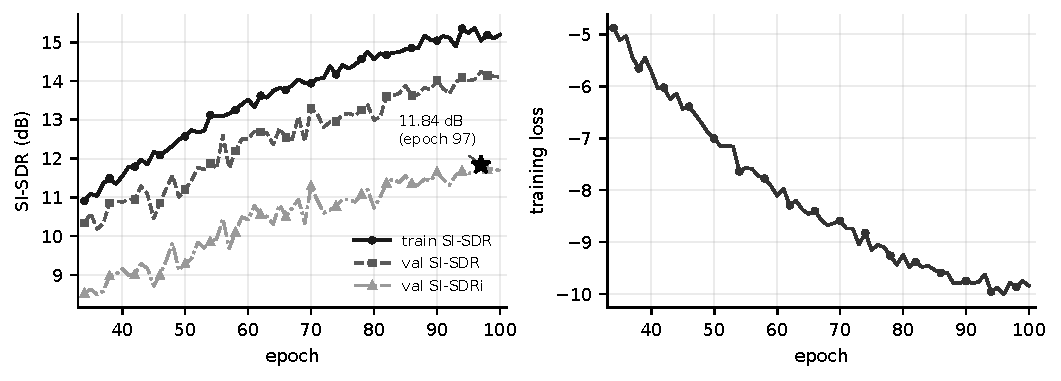
\includegraphics[width=\textwidth]{training_curves.pdf}
\caption{Training and validation \sisdr, validation \sisdri{} (star: best epoch) and the combined
loss for epochs 34--100.}
\label{fig:curves}
\end{figure}

%% ============================================================
%%  7. RESULTS
%% ============================================================
\section{Results}
\label{sec:results}

Training finished all 100 epochs. The best validation checkpoint
(\texttt{tse\_bsrnn\_big\_best.pt}) was reached at \textbf{epoch~97}, with a validation \sisdri{}
of \textbf{11.84\,dB} on unseen speakers. The fixed test set contains 1200 mixtures from 40 unseen
speakers.

The test \sisdr, STOI and PESQ numbers in this section come from a metrics file produced with an
\emph{earlier} best checkpoint, before training finished. They are historical results, not
final-checkpoint test results. Speaker confusion, the WER check, the efficiency measurements and
the six qualitative examples use the final checkpoint; on those six examples the final checkpoint
is 0.1--1.4\,dB better. A rerun with the epoch-97 checkpoint has not been completed, so
Tables~\ref{tab:test}, \ref{tab:scenario} and \ref{tab:difficulty}, plus Appendix
Table~\ref{tab:noiseenv}, remain earlier-checkpoint results. The final checkpoint is used only
where stated.

\subsection{Training progress}
After the resume at epoch~33 (validation \sisdri{} then 8.12\,dB), validation \sisdri{} rose from
8.5\,dB at epoch~34 to 11.7\,dB at epoch~100, with a best value of 11.84\,dB at epoch~97. The
training loss fell from $-4.9$ to $-9.8$ and training \sisdr{} from 10.9 to 15.2\,dB. Over the
last ten epochs the train--validation \sisdr{} gap averaged about 1.1\,dB, so there is no strong
overfitting. The curve flattens as the learning rate anneals towards $10^{-5}$: from epoch~90
onward, validation \sisdri{} stayed between 11.3 and 11.8\,dB. No batches were skipped for
non-finite loss in the final epochs. Swings of a few tenths of a dB from epoch to epoch are normal
because the validation set has only 300 mixtures.

\subsection{Test-set metrics}
\label{sec:testmetrics}
\Cref{tab:test} gives \sisdr, STOI and wideband PESQ on the test set with 95\% bootstrap
confidence intervals. The headline row group excludes the 65 clean-scenario items, where the
mixture already equals the reference.

\begin{table}[htbp]
\centering\small
\caption{Test metrics from the earlier checkpoint, mean with 95\% bootstrap CI. The headline
column excludes the 65 clean-scenario items.}
\label{tab:test}
\begin{tabular}{@{}lcc@{}}
\toprule
Metric & Non-clean ($n{=}1135$) & All items ($n{=}1200$)\\
\midrule
\sisdr{} input (dB) & 0.28 [0.00, 0.56] & 5.95 [4.62, 7.33]\\
\sisdr{} output (dB) & 11.06 [10.56, 11.56] & 12.72 [12.09, 13.34]\\
\textbf{\sisdri{} (dB)} & \textbf{10.78 [10.34, 11.21]} & 6.77 [5.73, 7.76]\\
STOI input & 0.772 [0.765, 0.780] & 0.785 [0.777, 0.792]\\
STOI output & 0.872 [0.863, 0.880] & 0.879 [0.870, 0.887]\\
PESQ output (wideband) & 2.20 [2.15, 2.24] & 2.33 [2.28, 2.38]\\
\bottomrule
\end{tabular}
\end{table}

On non-clean items the model improves \sisdr{} by 10.8\,dB and STOI by 0.10. The all-items
\sisdri{} of 6.77\,dB is lower purely because of the clean scenario (\Cref{tab:scenario}): there
the input \sisdr{} is about 105\,dB, so even a 41.6\,dB output \sisdr{} registers as a $-63$\,dB
``improvement''. That is a metric artefact rather than a quality problem. STOI is 1.00 and PESQ is
4.62 on clean items, so clean speech passes through almost unchanged.

\begin{table}[htbp]
\centering\small
\caption{Results by scenario from the earlier checkpoint. STOI is reported as input/output.}
\label{tab:scenario}
\begin{tabular}{@{}lrrrrrr@{}}
\toprule
Scenario & $n$ & \sisdr{} in & \sisdr{} out & \sisdri{} [95\% CI] & STOI in/out & PESQ\\
\midrule
noise & 290 & 4.22 & 17.73 & 13.51 [12.79, 14.23] & 0.90/0.95 & 2.89\\
speech & 294 & 1.15 & 10.81 & 9.65 [8.70, 10.56] & 0.76/0.88 & 2.29\\
speech\_noise & 551 & $-2.25$ & 7.68 & 9.93 [9.30, 10.52] & 0.71/0.83 & 1.78\\
clean & 65 & 104.86 & 41.64 & $-63.22$ [$-64.93$, $-61.67$] & 1.00/1.00 & 4.62\\
\bottomrule
\end{tabular}
\end{table}

Denoising alone (noise scenario) is easiest at 13.5\,dB. Removing a competing talker (speech,
9.7\,dB) and the hardest combination of talker plus noise (speech\_noise, 9.9\,dB) both give
around 10\,dB; the latter has the lowest output STOI (0.83) and PESQ (1.78). The \sisdri{} gain
also shrinks as input SNR rises, from about 13\,dB at low SNR to 9\,dB at high SNR, which is
expected because there is less noise left to remove; absolute quality (PESQ) improves with SNR.
The model does not collapse at hard ratios, and it still gains about 12\,dB at SIR below
$-3.3$\,dB and SNR below $-1.7$\,dB. Across the 16 DEMAND environments the mean \sisdri{} ranges
from 6.9\,dB (restaurant, \texttt{PRESTO}) to 17.8\,dB (washing, \texttt{DWASHING}); the hardest
environments are crowded or transit scenes. The full SIR/SNR and environment breakdowns are in
\Cref{app:breakdowns}.

\subsection{Qualitative examples}
Six test mixtures were drawn at random with a fixed seed and listened to. \Cref{tab:examples}
lists \sisdr{} before and after processing with the final checkpoint; all six improved by 11.3 to
21.4\,dB. \Cref{fig:spec} shows the spectrograms for the best of the six. These examples are
illustrative and do not replace the statistics above.

\begin{table}[htbp]
\centering\small
\caption{Randomly chosen test examples from the final checkpoint. The last column gives the change
relative to the earlier checkpoint.}
\label{tab:examples}
\begin{tabular}{@{}rrrrr@{}}
\toprule
Test index & Input \sisdr{} (dB) & Output \sisdr{} (dB) & Improvement (dB) & vs.\ earlier (dB)\\
\midrule
323 & $-3.50$ & 12.27 & $+15.77$ & $+1.35$\\
761 & 3.80 & 21.57 & $+17.77$ & $+0.25$\\
611 & 2.52 & 17.88 & $+15.36$ & $+1.00$\\
369 & $-0.77$ & 20.67 & $+21.44$ & $+0.52$\\
49 & 1.60 & 12.88 & $+11.27$ & $+0.51$\\
1016 & $-0.66$ & 11.38 & $+12.04$ & $+0.13$\\
\bottomrule
\end{tabular}
\end{table}

\begin{figure}[htbp]
\centering
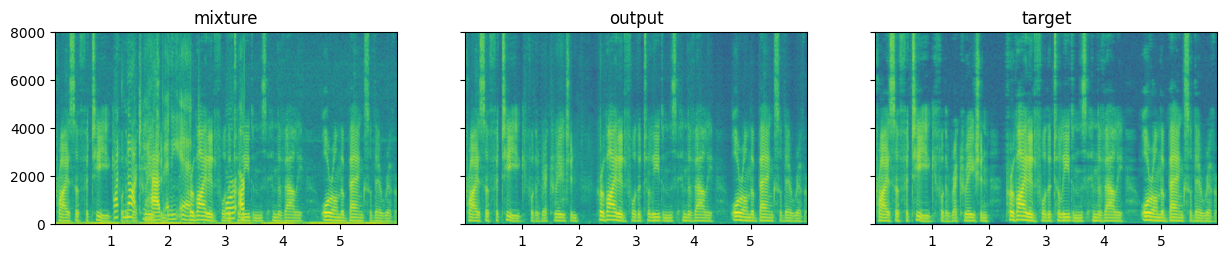
\includegraphics[width=\textwidth]{spec_ex369.png}
\caption{Test example 369 ($+21.4$\,dB, the best of the six): mixture (left), model output
(centre) and clean target (right). The competing voice and broadband noise are removed, and the
output closely resembles the target.}
\label{fig:spec}
\end{figure}

\subsection{Speaker confusion}
\label{sec:confusion}
The most characteristic TSE failure is extracting the \emph{wrong} speaker. For the 845 test
mixtures that contain an interferer we embedded the output, the clean target and a 5\,s segment of
the interferer with ECAPA-TDNN, and counted an output as confused when it is closer in cosine
similarity to the interferer than to the target. The confusion rate is \textbf{7.7\%} (65 of 845).
Mean similarity to the target rises from 0.584 for the mixture to 0.772 for the output.
\Cref{fig:confusion} (top) shows the two clusters and (bottom) the rate by condition: it is roughly
independent of SIR (6.5--8.3\%), slightly higher with added noise (about 8.4\% versus 6.5\%), and
clearly depends on enrollment length (about 2\% at 12\,s versus 8--13\% at 2--3\,s; values read
from the figure). Longer, cleaner enrollment is therefore the most effective lever against
confusion.

\begin{figure}[t]
\centering
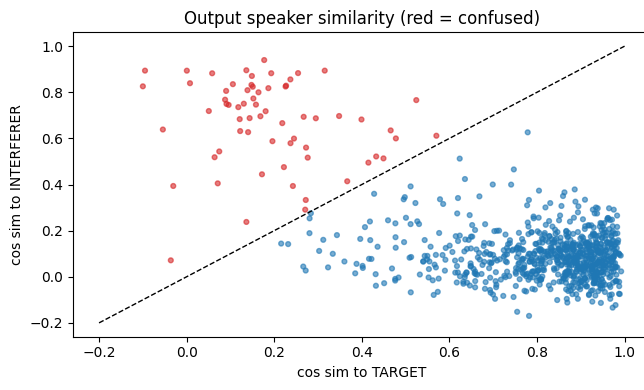
\includegraphics[width=0.62\textwidth]{speaker_similarity.png}\\[4pt]
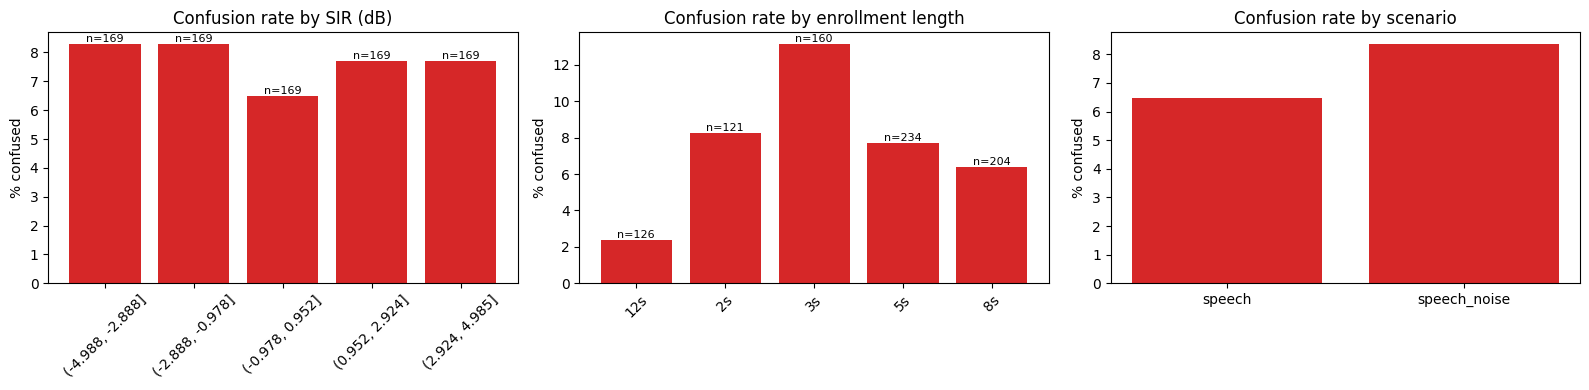
\includegraphics[width=\textwidth]{confusion_drivers.png}
\caption{Top: output similarity to the target versus the interferer (red points are confused
outputs). Bottom: confusion rate by SIR bin, enrollment length and scenario.}
\label{fig:confusion}
\end{figure}

\subsection{Downstream intelligibility}
\label{sec:wer}
To measure usefulness beyond signal metrics, 300 random test mixtures were transcribed with Whisper
\texttt{small.en} \cite{radford2023whisper}, using Whisper's transcript of the \emph{clean target} as
the reference rather than human transcripts, and WER was computed with \texttt{jiwer}.
\Cref{tab:wer} shows that extraction more than halves the WER.

\begin{table}[htbp]
\centering\small
\caption{Whisper WER (\%) on 300 test mixtures from the final checkpoint.}
\label{tab:wer}
\begin{tabular}{@{}lrrr@{}}
\toprule
Subset & $n$ & Mixture & Extracted\\
\midrule
All & 300 & 38.3 & \textbf{18.1}\\
Excluding clean & 285 & 40.2 & \textbf{18.9}\\
\midrule
noise & 77 & 7.0 & 5.8\\
speech & 77 & 40.4 & 10.5\\
speech\_noise & 131 & 60.0 & 31.9\\
clean & 15 & 0.0 & 0.0\\
\bottomrule
\end{tabular}
\end{table}

The largest gain is with a competing talker: WER drops from 40.4\% to 10.5\% for speech and from
60.0\% to 31.9\% for speech plus noise. Noise-only mixtures are already easy for Whisper (7.0\%),
and clean speech is not damaged (0\% WER).

Additional diagnostics come from both checkpoints. The earlier checkpoint improves \sisdr{} on
88.3\% of the 1200 test mixtures, and its \sisdri{} correlates strongly negatively with input
\sisdr{} ($r=-0.90$), weakly negatively with SNR ($r=-0.21$) and SIR ($r=-0.11$), and essentially
not with enrollment duration ($r=0.05$). For the 845 mixtures with an interferer, the final
checkpoint gives a mean \sisdri{} of 11.19\,dB when the output matches the target speaker and
$-6.40$\,dB when it does not. The final-checkpoint relative WER reduction is 52.9\%.

\subsection{Efficiency}
\label{sec:eff}
\Cref{tab:eff} reports inference cost on an NVIDIA L4 for a 6\,s clip, processed offline in one
pass.

\begin{table}[htbp]
\centering\small
\caption{Model size and inference cost for a 6\,s clip, batch 1, on an NVIDIA L4.}
\label{tab:eff}
\begin{tabular}{@{}lrr@{}}
\toprule
 & fp32 & fp16 autocast\\
\midrule
Parameters & \multicolumn{2}{c}{16.83\,M}\\
Compute & \multicolumn{2}{c}{23.87\,GMACs per clip (3.98\,GMACs per second of audio)}\\
Time per clip & 164.9\,ms & 181.1\,ms\\
Offline RTF & 0.0275 & 0.0302\\
Peak GPU memory & 1057\,MiB & 870\,MiB\\
\bottomrule
\end{tabular}
\end{table}

The fp32 pass takes 164.9\,ms for this 6\,s clip; fp16 saves memory but is slower at batch size
one. These are offline GPU measurements. They do not imply low latency: the bidirectional LSTMs
need the whole clip, and CPU speed has not yet been measured.

%% ============================================================
%%  8. LIMITATIONS
%% ============================================================
\section{Challenges and Limitations}
\label{sec:limits}

\begin{itemize}
  \item \textbf{Non-causal model.} Bidirectional LSTMs use future frames, so the current model
        cannot run with low latency. This departs from the proposal's low-latency goal, and a
        causal variant has not been built.
  \item \textbf{Size and compute.} At 16.83\,M parameters and about 4\,GMACs per second of audio,
        the model is not yet compatible with the compact CPU target. CPU speed is unmeasured, and
        the reported RTF is an offline GPU figure.
  \item \textbf{Speaker confusion.} In 7.7\% of interferer mixtures the output matches the
        interferer better than the target, mostly with 2--3\,s enrollments
        (\Cref{sec:confusion}). Target-absent behaviour is untested, so the system may extract the
        wrong voice when the target is silent.
  \item \textbf{No unseen-noise test.} DEMAND recordings are split by time, so the same 16
        environments appear in training, validation and test. Performance on unseen noise types is
        therefore not demonstrated. Reverberation is also absent from both training and test.
  \item \textbf{Enrollment diversity.} Enrollments are VAD-cleaned from clean recordings, with
        only 10 recipes per training speaker. Real enrollments are noisier. The same energy VAD is
        used for the cached banks and for a user's own recording, as described in
        \Cref{sec:system}.
  \item \textbf{Length mismatch.} Training uses 4\,s clips and evaluation 6\,s clips. Long inputs
        are processed in one pass or in 30\,s chunks without overlap-add, which may cause boundary
        artefacts.
  \item \textbf{Evaluation status.} The 300-mixture validation set is small. The test
        \sisdr/STOI/PESQ tables were computed with an earlier checkpoint and must be rerun for the
        final model. The clean scenario distorts the aggregate \sisdri, so non-clean results are
        the headline.
  \item \textbf{WER reference.} The WER check uses Whisper transcripts of the clean target as the
        reference, not human transcripts, and covers 300 mixtures.
  \item \textbf{Reproducibility.} The configured random seed is not applied inside the training
        loop, and dataset workers use unseeded generators, so reruns see different sampled
        mixtures.
\end{itemize}

%% ============================================================
%%  9. REMAINING WORK
%% ============================================================
\section{Remaining Work and Revised Plan}
\label{sec:remaining}

Table~\ref{tab:plan} lists the remaining tasks with a primary owner and a priority. Three items
are high priority: rerunning the test metrics with the epoch-97 checkpoint, the conditioning
ablation promised in the proposal, and a test on unseen noise environments. CPU efficiency and a
causal variant are medium priority and depend on the time left after the high-priority items.

\begin{table}[H]
\centering\small
\caption{Remaining work and primary owner. Ownership follows the proposal's module assignments.}
\label{tab:plan}
\begin{tabularx}{\textwidth}{@{}>{\raggedright\arraybackslash}p{4.1cm} Y >{\raggedright\arraybackslash}p{2.5cm} l@{}}
\toprule
\textbf{Task} & \textbf{Description} & \textbf{Owner} & \textbf{Priority}\\
\midrule
Final-checkpoint evaluation & Rerun \sisdri, STOI and PESQ (plus PESQ of the unprocessed mixture)
  with the epoch-97 checkpoint and refresh all breakdowns & Sostika & High\\
Conditioning ablation & Compare additive-only, FiLM-only and concatenation/gating, as promised in
  the proposal & Prashamsa & High\\
Unseen-noise test & Hold out whole DEMAND environments, or add MUSAN or self-recorded noise, for
  testing & Austina & High\\
Efficiency measurement & RTF, latency and memory on CPU (GPU RTF 0.028 already measured) & Sostika & Medium\\
Model compression and causal variant & Smaller configuration; unidirectional LSTM and causal STFT
  if time permits & Prashamsa, Sostika & Medium\\
Generalisation additions & Reverberation (RIRs), noisy and longer enrollments to cut speaker
  confusion, target-absent samples & Austina & Medium\\
Demo and documentation & Packaged inference script or small demo, final report and presentation &
  All & High\\
\bottomrule
\end{tabularx}
\end{table}

%% ============================================================
%%  10. CONCLUSION
%% ============================================================
\section{Conclusion}
We moved from the proposal's causal Conv-TasNet design to a speaker-conditioned BSRNN, and
training is complete. The model reached a validation \sisdri{} of 11.84\,dB on unseen speakers. In
the earlier-checkpoint test evaluation, non-clean \sisdr{} improved by about 10.8\,dB and STOI
rose from 0.77 to 0.87; the final-checkpoint WER check fell from 38.3\% to 18.1\%. The trade-off
is clear: the current model is larger and non-causal, and 7.7\% of interferer mixtures were
classified as speaker confusions. We still need the final test-metric rerun, the conditioning
ablation, an unseen-noise test and CPU measurements. On the team side, Austina led data
preparation, Prashamsa led the speaker encoder and conditioning work, and Sostika led training
and inference; all three shared the literature review, evaluation and writing.

%% ============================================================
%%  REFERENCES
%% ============================================================
\bibliographystyle{ieeetr}
\setlength{\bibsep}{2pt}
\bibliography{references}

%% ============================================================
%%  APPENDIX
%% ============================================================
\appendix

\section{Reproducibility Notes}
\label{app:repro}
\begin{itemize}
  \item \textbf{Code:} \texttt{tselib.py} contains the model, sampler, datasets, loss and training
        loop, with two YAML configuration files. These are kept on Google Drive under
        \texttt{tse-project/}. The project repository is at
        \url{https://github.com/frecklehead/SIC-AI-Project}.
  \item \textbf{Training notebook:} downloads LibriSpeech and DEMAND, loads manifests and cached
        embedding banks, patches gradient checkpointing, and calls \texttt{T.train(\ldots)}.
  \item \textbf{Test notebook:} loads the best checkpoint, plays the mixture, output and target,
        computes \sisdr, STOI and PESQ on the test manifest, and separates user-supplied files.
  \item \textbf{Software:} PyTorch 2.x (CUDA), SpeechBrain, \texttt{pystoi}, \texttt{pesq},
        \texttt{jiwer} and Whisper through \texttt{transformers} for the WER check.
  \item \textbf{Analysis cells:} per-scenario, SNR, SIR and noise-environment breakdowns, bootstrap
        confidence intervals, speaker-confusion analysis, WER and FLOP/RTF benchmarking are in the
        training notebook after the test-loading cell.
\end{itemize}

\section{Additional Test Breakdowns}
\label{app:breakdowns}

\begin{table}[htbp]
\centering\footnotesize
\caption{\sisdri{} (dB) by difficulty from the earlier checkpoint. SIR bins use the 845 mixtures
with an interferer; SNR bins use the 841 mixtures with noise.}
\label{tab:difficulty}
\begin{tabular}{@{}lrrr@{\hspace{1.2cm}}lrrr@{}}
\toprule
SIR bin (dB) & $n$ & \sisdri{} & PESQ & SNR bin (dB) & $n$ & \sisdri{} & PESQ\\
\midrule
$[-5.0,-3.3]$ & 131 & 11.98 & 1.81 & $[-5.0,-1.7]$ & 155 & 12.86 & 1.77\\
$(-3.3,-1.7]$ & 152 & 9.03 & 1.80 & $(-1.7,1.7]$ & 136 & 13.05 & 2.05\\
$(-1.7,0.0]$ & 134 & 10.57 & 1.91 & $(1.7,5.0]$ & 142 & 11.75 & 2.22\\
$(0.0,1.7]$ & 147 & 10.22 & 1.99 & $(5.0,8.3]$ & 135 & 10.83 & 2.31\\
$(1.7,3.3]$ & 144 & 8.42 & 2.05 & $(8.3,11.6]$ & 126 & 9.05 & 2.27\\
$(3.3,5.0]$ & 137 & 9.03 & 2.19 & $(11.6,14.9]$ & 147 & 9.20 & 2.42\\
\bottomrule
\end{tabular}
\end{table}

\begin{table}[htbp]
\centering\footnotesize
\caption{Mean \sisdri{} and output quality per DEMAND environment from the earlier checkpoint
(mixtures containing noise only).}
\label{tab:noiseenv}
\begin{tabular}{@{}lrrrr@{\hspace{0.8cm}}lrrrr@{}}
\toprule
Env. & $n$ & \sisdri{} & STOI & PESQ & Env. & $n$ & \sisdri{} & STOI & PESQ\\
\midrule
DKITCHEN & 57 & 13.87 & 0.92 & 2.56 & OOFFICE & 48 & 13.22 & 0.89 & 2.35\\
DLIVING & 61 & 9.14 & 0.85 & 1.79 & PRESTO & 49 & 6.87 & 0.79 & 1.64\\
DWASHING & 33 & 17.76 & 0.92 & 2.77 & PSTATION & 64 & 8.56 & 0.84 & 1.97\\
NFIELD & 44 & 12.86 & 0.88 & 2.26 & SPSQUARE & 49 & 9.45 & 0.85 & 1.93\\
NPARK & 52 & 11.14 & 0.85 & 1.90 & STRAFFIC & 51 & 10.48 & 0.89 & 2.27\\
NRIVER & 44 & 12.01 & 0.86 & 2.08 & TBUS & 63 & 13.38 & 0.92 & 2.62\\
OHALLWAY & 53 & 13.40 & 0.88 & 2.33 & TCAR & 52 & 13.52 & 0.92 & 2.82\\
OMEETING & 65 & 8.38 & 0.83 & 1.82 & TMETRO & 56 & 8.34 & 0.83 & 1.81\\
\bottomrule
\end{tabular}
\end{table}

\end{document}
